\documentclass[12pt]{article}
\usepackage{amsmath}
\usepackage{appendix}
\usepackage{enumerate}
\usepackage[top=1in,bottom=1in,left=1in,right=1in]{geometry}
\usepackage{graphicx}
\usepackage{subfigure}
\usepackage{multicol}

\newcommand{\betan}{ $\beta_{n}$ }
\newcommand{\qbeta}{Q$_\beta$}
\newcommand{\qbetan}{Q$_{\beta-n}$}

\newcommand{\diff}[3][]{
  \ensuremath{\frac{\mathrm{d}^{#1} {#2}}{\mathrm{d} {#3}^{#1}}}}

\newcommand{\pdiff}[3][]{
  \ensuremath{\frac{\partial^{#1} {#2}}{\partial {#3}^{#1}}}}


\title{Cascade Builder}
\author{S. V. Paulauskas}
\date{\today}

\begin{document}
\maketitle
\section{Pseudo-code}
\begin{eqnarray} 
  &&\forall \hat{G} \in \bigcirc \\
  &&BB[G, SS=\bigcirc,\hat{G}]\\
  &&\quad \text{IF } H \ni HH \rightarrow \mathrm{continue} \\
  &&\quad NSS = SS \cap NC \\
  &&\quad \text{IF } NSS = \emptyset \rightarrow C=C \cup H, \mathrm{continue} \\  
  &&\quad \forall \hat{G} \in NSS \\
  &&\quad \quad NH = H \cup \hat{G} \\
  &&\quad \quad \text{IF } CC[NH] \rightarrow BB[NH, NSS, \hat{G}], HH = HH \cup NH
\end{eqnarray}
Where the variables with a hat are doubles, $\bigcirc$ is the world, BB is the 
branch builder routine, G is the set of gammas in the system, SS is the search 
set, H is the search history, HH is the history of histories, NSS is the new 
search set, NC are the current gamma's coincidences, C is the set of cascades, 
NH is the new history, CC is the coincidence check.
\textbf{Special thanks to the Awesome D. Miller}
\section{Test Level Schemes}
For both of the following tests assume that the intensity of the gamma 
increases with increasing subscript. 
\subsection {Test 00}
In this test 7 is the only gamma that does not have a coincidence, and there 
was a false positive with 7 and 1.
\begin{figure} [t]
  \begin{center}
    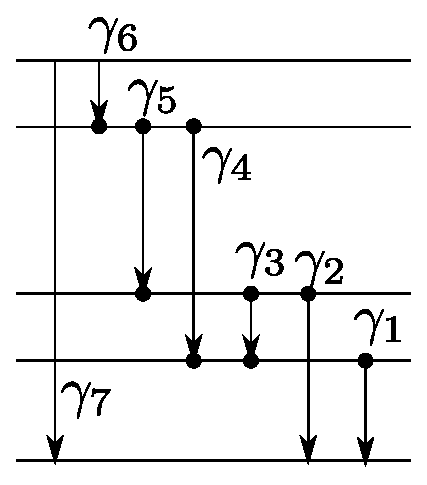
\includegraphics{../pictures/test00.eps}
    \caption{This is the level scheme for Test00.}
    \label{fig:test00}
  \end{center}
\end{figure}
\subsubsection{Coincidence Information}
\begin{multicols}{2}
\begin{description}
\item[1: ] 3, 4, 5, 6
\item[2: ] 5, 6 
\item[3: ] 1, 5, 6 
\item[4: ] 1, 6 
\item[5: ] 1, 2, 3, 6
\item[6: ] 1, 2, 3, 4, 5
\item[7: ] 1
\end{description}
\end{multicols}
\subsubsection{Cascades}
\begin{enumerate}
\item 1, 3, 5, 6
\item 1, 4, 6
\item 2, 5, 6
\end{enumerate}
\subsection{Test01}
This test has 15 gammas in it. The first 9 gammas are the gammas seen in the 
$^{81}$Zn decay, built by S. Padgett. The remaining gammas were added to create 
more complicated cascades.
\begin{figure} [t]
  \begin{center}
    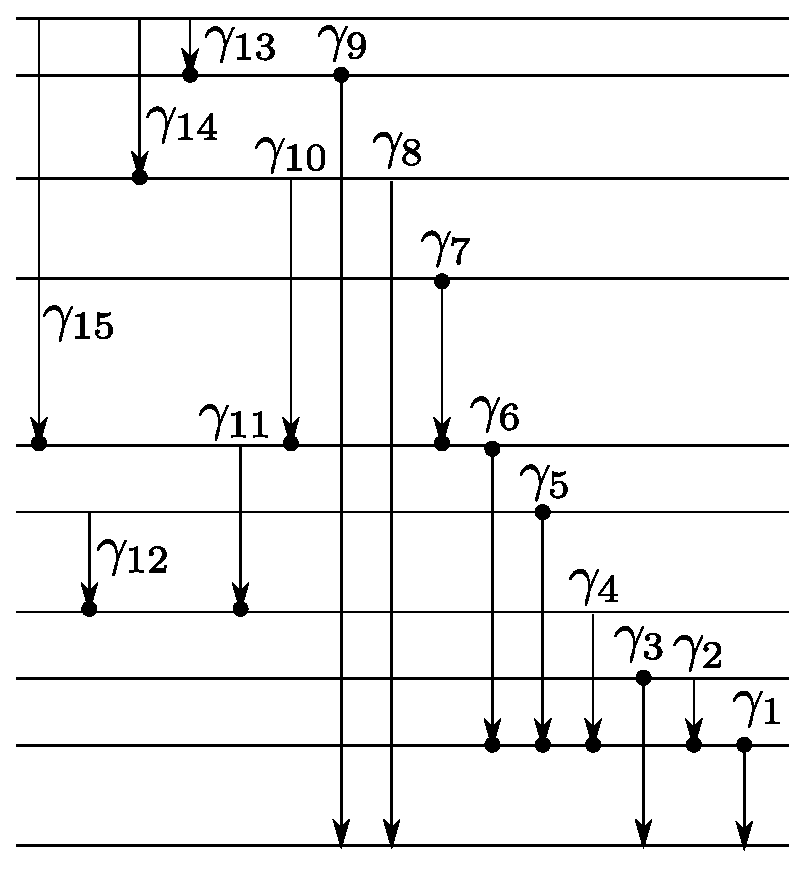
\includegraphics[width=4.5in]{../pictures/test01.eps}
    \caption{This is the level scheme for Test01.}
    \label{fig:test01}
  \end{center}
\end{figure}
\subsubsection{Coincidence Information}
\begin{multicols}{2}
\begin{description}
\item[1: ] 2, 4, 5, 6, 7, 10, 14, 15
\item[2: ] 1
\item[3: ] 11, 12
\item[4: ] 1
\item[5: ] 1, 10, 15
\item[6: ] 1, 7, 14
\item[7: ] 1, 6, 14
\item[8: ] 1
\item[9: ] 13
\item[10: ] 1, 5
\item[11: ] 3
\item[12: ] 2, 3
\item[13: ] 9
\item[14: ] 1, 6, 7
\item[15: ] 1, 5, 11
\end{description}
\end{multicols}
\subsubsection{Cascades}
\begin{multicols}{2}
\begin{enumerate}
\item 1, 2
\item 1, 4
\item 1, 5, 10
\item 1, 5, 15
\item 1, 6, 7, 14
\item 3, 11
\item 3, 12
\item 9, 13
\item 8
\end{enumerate}
\end{multicols}

\subsection{Test02}
This is a partial level scheme for $^{194}$Hg.
%\begin{figure} [t]
%  \begin{center}
%    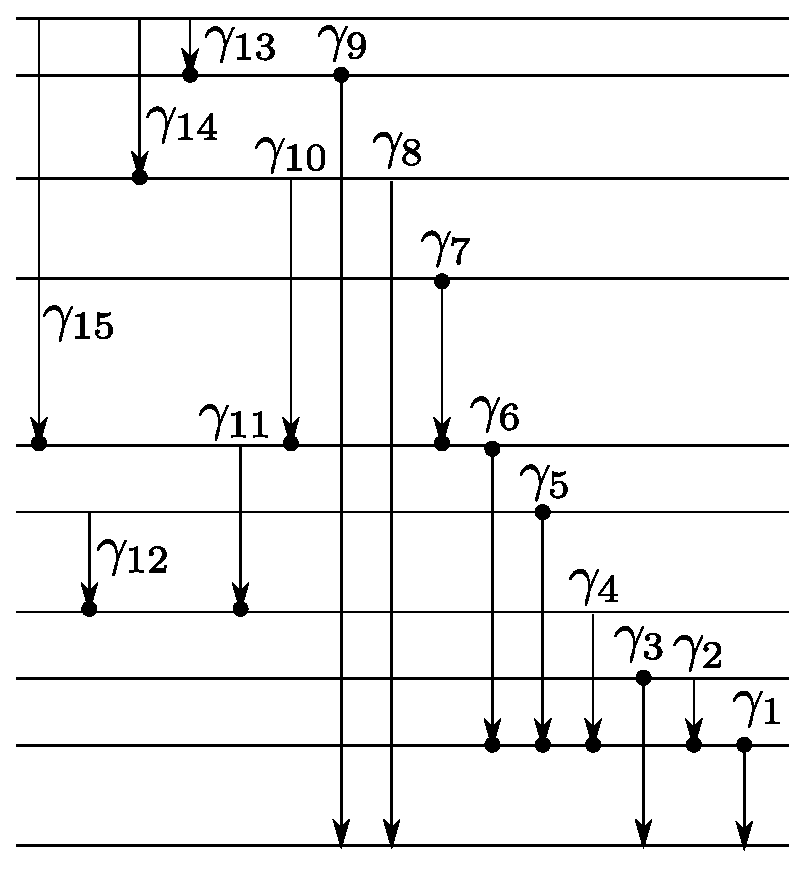
\includegraphics[width=4.5in]{../pictures/test01.eps}
%    \caption{This is the level scheme for Test01.}
%    \label{fig:test01}
%  \end{center}
%\end{figure}
\subsubsection{Coincidence Information}
\begin{multicols}{2}
\begin{description}
\item[97: ] 227, 232, 280, 418, 427, 485, 544, 636, 706, 748
\item[227: ] 97, 427, 636, 748
\item[232: ] 97, 280, 418, 427, 485, 544, 636, 706, 734, 748, 1799
\item[280: ] 97, 232, 427, 636, 734, 748, 1799
\item[418: ] 97, 232, 427, 636, 734, 748, 1799
\item[427: ] 97, 227, 232, 280, 418, 485, 544, 565, 636, 706, 734, 748, 1799
\item[485: ] 97, 232, 427, 544, 636, 734, 748, 1799
\item[544: ] 97, 232, 427, 485, 636, 706, 734, 748, 1799
\item[565: ] 427, 636, 734
\item[636: ] 97, 227, 232, 280, 418, 427, 485, 544, 565, 706, 734, 748, 1799
\item[706: ] 97, 232, 427, 544, 636, 734, 748, 1799
\item[734: ] 232, 280, 418, 427, 485, 544, 565, 636, 706, 1799
\item[748: ] 97, 227, 232, 280, 418, 427, 485, 544, 636, 706
\item[1799: ] 232, 280, 418, 427, 485, 544, 636, 706, 734
\end{description}
\end{multicols}
\subsubsection{Cascades}
\begin{multicols}{2}
\begin{enumerate}
\item 280, 232, 97, 748, 636, 427
\item 280, 232, 1799, 734, 636, 427
\item 565, 734, 636, 427
\item 706, 544, 232, 97, 748, 636, 427
\item 706, 544, 232, 1799, 734, 636, 427
\item 485, 544, 232, 97, 748, 636, 427
\item 485, 544, 232, 1799, 734, 636, 427
\item 418, 232, 97, 748, 636, 427
\item 418, 232, 1799, 734, 636, 427
\item 227, 97, 748, 636, 427
\end{enumerate}
\end{multicols}

\bibliographystyle{naturemag}
\bibliography{/home/vincent/research/publicationWork/ReferenceList}
\end{document}
